\documentclass[10pt,a4paper]{article}
\usepackage[a4paper,rmargin=3cm, lmargin=2.5cm, tmargin=2.5cm, bmargin=3cm]{geometry}
\usepackage{graphicx}
\usepackage{indentfirst}
\usepackage[brazilian]{babel}
\usepackage[utf8]{inputenc}
\usepackage[table,xcdraw]{xcolor}
\usepackage[T1]{fontenc}
\usepackage{pgfplots}
\usepackage{multicol}
\usepackage{times}
\usepackage{tikz}
\usepackage{float}
\usepackage[outdir=./]{epstopdf}
\usepackage{fancyhdr}
\usepackage{mathtools}
\DeclarePairedDelimiter\ceil{\lceil}{\rceil}
\DeclarePairedDelimiter\floor{\lfloor}{\rfloor}

\renewcommand{\headrulewidth}{0pt}
\usepackage[backend=bibtex, bibencoding=ascii, style=authoryear, firstinits=true]{biblatex}
\addbibresource{Artigo.bib}
\thispagestyle{fancy}
\fancyhead[C]{\includegraphics[scale=0.06]{img/LogoUnifei}}


\usepackage{etoolbox}
\appto\normalsize{\belowdisplayshortskip=\belowdisplayskip}
% the following two are not strictly necessary
\appto\small{\belowdisplayshortskip=\belowdisplayskip}
\appto\footnotesize{\belowdisplayshortskip=\belowdisplayskip}

\setlength{\parskip}{0pt}
\raggedcolumns

\title{Desenvolvimento de uma babá eletrônica com reconhecimento de choro infantil utilizando redes neurais artificiais}
\author{Gustavo S. Leal}
\date{\today}

\makeatletter

\begin{document}
\begin{center}

{\large Universidade Federal de Itajubá}

{\scriptsize Graduação em Engenharia Eletrônica}

\vspace{1.25cm}

\textsc{\textbf{\@title}}	
\vspace{0.5cm}

\textsc{\@author}

\vspace{0.35cm}

\textit{Orientador:}

\textsc{Giscard F. C. Veloso}

\vspace{0.75cm}
\textit{Instituto de Engenharia de Sistemas e Tecnologia da Informação, Universidade Federal de Itajubá}

\textit{Av. BPS 1303, 37500-903, Itajubá, MG, Brasil}

\textit{E-mail}: \texttt{gustavo.soares.leal@gmail.com}
\end{center}

\vspace{0.75cm}

{\footnotesize \textbf{Abstract---} 
This article presents the development process of a infant cry monitoring device which is capable of recognizing a cry event and alert a carer remotely. The system operates by extracting mel-frequency cepstral coefficients (MFCC), which are used as characteristics for an artificial neural network-based classification. The system consists of two units: a transmitter (central) and a receptor. The transmitter is responsible for sound capturing, its digital processing and classification using artificial neural networks. The receptor is a device that receives a signal from the transmitter, triggering vibrating, sound and visual alerts.
}
\vspace{0.35cm}

{\footnotesize \textbf{Keywords---} mfcc, neural networks, digital signal processing, cepstrum, hardware.}
\vspace{0.35cm}

{\footnotesize \textbf{Resumo---}
Este artigo apresenta o processo de desenvolvimento de um dispositivo para monitoramento de choro infantil capaz de reconhecer um evento de choro e alertar remotamente um responsável. O sistema opera realizando a extração de coeficientes cepstrais na frequência mel (MFCC), que são utilizados como características para a classificação baseada em redes neurais artificiais. O sistema é constituído por duas unidades: um transmissor (central) e um receptor. O transmissor é responsável pela captação sonora, seu processamento digital e sua classificação utilizando redes neurais artificais. O receptor é um dispositivo que recebe um sinal do transmissor, disparando alertas vibratórios, sonoros e visuais.}


\vspace{0.35cm}
{\footnotesize \textbf{Palavras chave---} mfcc, redes neurais, processamento digital de sinais, cepstrum, hardware.}
\vspace{0.35cm}

\begin{multicols*}{2}

\section{Introdução}
Segundo o censo demográfico de 2010 (\cite{censo2010}), no Brasil, 5,1\% da população possui algum tipo de deficiência auditiva.  Dois milhões de pessoas declararam ser completamente surdas (não conseguem ouvir de modo algum) ou responderam ter grande dificuldade de audição.

Em particular, o caso de pais surdos desperta a atenção quanto ao relacionamento e ao cuidado com seus bebês.

Atualmente, há dispositivos eletrônicos comercializados para monitoramento de crianças, como a chamada babá eletrônica. Este tipo de dispositivo, em sua maioria, confia na reprodução remota do som ambiente do recinto onde está uma criança. Os responsáveis são alertados quando escutam os sons emitidos. Este tipo de dispositivo, uma vez que baseia-se apenas na transmissão de informação sonora, não pode ser usado por indivíduos surdos.

Este trabalho apresenta o desenvolvimento de um sistema embarcado capaz de detectar choro infantil, diferenciando-o de outros sons no ambiente, e enviar, remotamente, um alerta vibratório para um dispositivo remoto, funcionando assim como uma babá eletrônica com foco principal em usuários surdos ou com dificuldade de audição.

O projeto inclui o desenvolvimento de hardware e software, desde a escolha de componentes e o projeto da placa de circuito impresso, até o desenvolvimento do software, responsável por todo o processamento, que será embarcado na placa.

A figura \ref{fig:sistema_blocos} apresenta um diagrama de blocos simplificado do sistema proposto.


% Tikz
\tikzstyle{startstop} = [rectangle, rounded corners, minimum width=2cm, minimum height=1cm,text centered, draw=black, fill=none]
\tikzstyle{arrow} = [thick,->,>=latex]
\tikzstyle{rfarrow} = [thick,->,>=latex,decorate,decoration={snake,amplitude=.6mm,segment length=3mm,post length=1mm}]


\begin{figure*}
\centering
\resizebox{0.7\textwidth}{!}{%
\begin{tikzpicture}[thick, node distance=2.5cm]	
				
		\node (micro) [startstop] {$\mu$C};
	\node (radio) [startstop, left of=micro, xshift=-1cm] {Rádio};
	\node (mic) [startstop, below of=micro] {Microfone};
	\node (supply) [startstop, above of=micro] {Alimentação};
	\node (radio2) [startstop, left of=radio,xshift=-2cm] {Rádio};
	\node (micro2) [startstop, left of=radio2,xshift=-1cm] {$\mu$C};
		
	\node (supply2) [startstop, above of=micro2] {Alimentação};
	\node (alerta) [startstop, below of=micro2] {Alerta};
	\draw [arrow] ([yshift=1ex]micro.west) -- node[anchor=south] {SPI} ([yshift=1ex]radio.east);
	\draw [arrow] ([yshift=-1ex]radio.east) -- ([yshift=-1ex]micro.west);
						
	\draw [arrow] ([yshift=1ex]micro2.east) -- node[anchor=south] {SPI} ([yshift=1ex]radio2.west);
	\draw [arrow] ([yshift=-1ex]radio2.west) -- ([yshift=-1ex]micro2.east);
	
	\draw [arrow] (supply2.south) -- (micro2.north);
	\draw [arrow] (micro2.south) -- (alerta.north);				

	\draw [arrow] (mic.north) -- (micro.south);
	\draw [arrow] (supply.south) -- (micro.north);
	\draw [rfarrow] (radio.west) -- node[anchor = south] {RF} (radio2.east);						
					
\end{tikzpicture}
}%
\caption{Diagrama de blocos do sistema proposto}
\label{fig:sistema_blocos}	
\end{figure*}

\section{Características do choro infantil}
De acordo com (\cite{brazelton1962}), o choro infantil é fisiologicamente útil nos primeiros dias de vida, sendo necessário para sua sobrevivência. O choro serve como ajuda na organização da função cardiorespiratória dos bebês.
Ainda segundo (\cite{brazelton1962}), logo após o nascimento, o choro começa a agir como resposta a necessidades fisiológicas, como fome ou desconforto.

	(\cite{truby1965}) classificaram como \textit{choro básico} infantil aquele em que a criança não demonstra grande desconforto, podendo apresentar frequências fundamentais de 400 a 550 Hz e uma característica suave.

Um segundo tipo de choro apresenta característica disfônica, onde ocorrem oscilações e deformações das vias aéreas superiores, gerando um som definido como rouco ou áspero, com oscilações mensuradas em torno de 130 Hz.

Ainda, o último tipo de choro apresentado é descrito como aquele onde existe uma impressão de um som de frequência extremamente alta. Nas gravações realizadas, um choro com frequência fundamental de 400 Hz alterava-se abruptamente para 1400 Hz.

A figura \ref{fig:fftchoro} apresenta o conteúdo espectral de uma amostra de choro infantil.

\begin{figure}[H]
\centering
\includegraphics[width=0.33\textwidth]{img/fftGraph}
\caption{Conteúdo espectral de uma amostra de choro infantil}
\label{fig:fftchoro}
\end{figure}
		
\section{Audição humana e percepção psicológica de tons}
\subsection{Audição humana}

O ouvido humano é constituído por estruturas responsáveis por captar vibrações do ar e transmiti-las ao cérebro. 

No ouvido externo está localizado o canal auditivo, um pequeno tubo que se estende em direção à cabeça. Sua função é direcionar o som ambiente para os ouvidos médio e interno, que se localizam dentro do crânio. Na extremidade final do canal auditivo está o tímpano, uma fina camada que vibra quando atingida pelas ondas sonoras.

O ouvido médio constitui-se de pequenos ossos que transferem a vibração do tímpano para a cóclea, localizada no ouvido interno. (\cite{smith1999dsp})

A cóclea é uma pequena estrutura espiral que possui um líquido em seu interior. O movimento do líquido coclear causado pelas vibrações deforma a membrana basilar. As características destas deformações dependem da região atingida da membrana, conferindo-a a capacidade de distinguir diferentes frequências. (\cite{purves2001neuroscience})

\subsection{Escala de frequência mel}
A escala de frequência mel tenta mensurar a sensação psicológica proporcionada pelo ouvido humano a cada tom. 

(\cite{stevens1937}) construíram uma escala baseada na comparação de tons. Seu nome é oriundo da palavra \textit{\textbf{mel}odia}. 

Para a constituição da escala, realizou-se um experimento onde os participantes ouviam um tom em uma frequência fixa e deveriam selecionar a frequência de um próximo tom de forma que este soasse como a metade do valor daquele.

A escala foi construída a partir da referência de que um tom de 1000Hz teria o valor de 1000 mels. Os demais tons foram determinados pelos participantes do experimento e a fórmula utilizada para conversão (\cite{oshaughnessy1987}) é dada por

\begin{equation}
 m = 2595 log(1+\frac{f}{700})
\end{equation}
e, inversamente
\begin{equation}
f = 700(10^{\frac{m}{2595}}-1)
\end{equation}
onde $ f $ é a frequência em hertz e $ m $ a frequência (ou tom) em mels. Esta relação é apresentada na figura \ref{fig:hzmels}.

\begin{figure}[H]
	\centering\includegraphics[width=0.4\textwidth]{img/hzmels}
	\caption{Relação entre escalas mel e Hz}
	\label{fig:hzmels}
\end{figure}


\section{Coeficientes cepstrais na frequência mel (MFCC)}

Os coeficientes cepstrais na frequência mel (\textit{MFCC - Mel Frequency Cepstral Coefficients}) são coeficientes obtidos a partir do \textit{cepstrum mel}, onde, na obtenção do cepstrum, utiliza-se a escala de frequência mel. (\cite{davis1980})
\newline Estas características são largamente utilizadas em aplicações de reconhecimento de voz (\cite{benesty2007springer}), mas também encontram aplicações em detecção de choro infantil (\cite{cohen2012}).
				
A implementação (\cite{mfcc_implementation}) para obtenção destes coeficientes, representada no diagrama de blocos da figura \ref{fig:algoritmomfcc}, começa pela divisão de um sinal discreto no tempo em \textit{frames} entre 20 a 40 milissegundos de duração.
			
Para cada um destes \textit{frames} (mostrados na figura \ref{fig:frames}), toma-se a transformada discreta de Fourier (DFT) das amostras, seguido pela densidade espectral, onde toma-se o valor absoluto do resultado da DFT, elevando-o ao quadrado e dividindo pelo número de amostras do sinal.
\newline O resultado passa por um banco de filtros passa-banda - como o mostrado na figura \ref{filterbank_graph} - gerados a partir da conversão de mel em hertz. Esta divisão é feita para avaliar padrões de distribuição de energia ao longo do espectro.
\begin{figure}[H]
	\centering\includegraphics[width=0.5\textwidth]{img/filterbank_new}
	\caption{Banco de filtros passa-banda}
	\label{filterbank_graph}
\end{figure}

Soma-se, então, o resultado da aplicação de cada um destes filtros (chamado \textit{energia}) individualmente.
\newline Toma-se o logaritmo das energias acima obtidas, seguido pela transformada cosseno discreta (DCT). Os valores resultantes são os coeficientes desejados. É comum, na maioria das aplicações, manter os 13 primeiros coeficientes, por terem maior informação na faixa de frequência da voz humana. Neste trabalho, portanto, estes 13 coeficientes foram utilizados como entrada para a rede neural. (\cite{mfcc_implementation})

\begin{figure}[H]
	\centering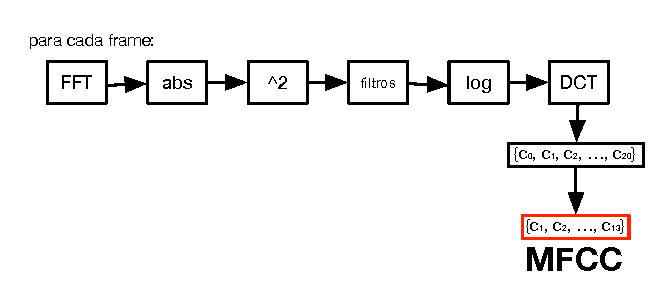
\includegraphics[width=0.4\textwidth]{../Diagramas/AlgoritmoMFCC}
	\caption{Diagrama de blocos do algoritmo para extração dos coeficientes}
	\label{fig:algoritmomfcc}
\end{figure}

Para a aplicação proposta, utilizou-se uma frequência de amostragem de 10 kHz. O conversor analógico digital adquire 1280 amostras e as armazena em um vetor, posteriormente dividindo-o em \textit{frames} de 25,6 ms de duração (correspondentes a 256 amostras) com 64 amostras sobrepostas. A sobreposição de amostras é feita para diminuir a perda de informações causadas pela aplicação de uma janela antes do processamento da FFT. 

\begin{figure}[H]
	\centering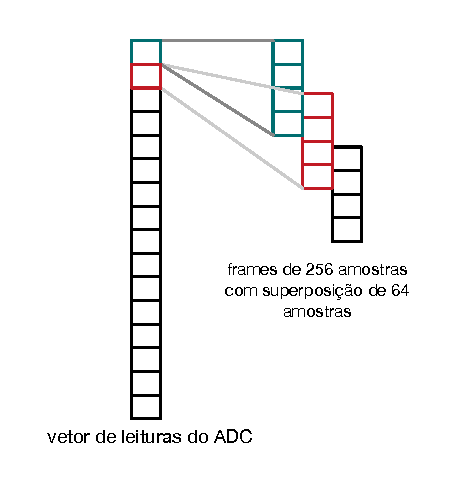
\includegraphics[width=0.5\textwidth]{../Diagramas/FramesMFCC}
	\caption{Representação da divisão em \textit{frames}}
	\label{fig:frames}
\end{figure}


As operações foram efetuadas utilizando aritmética de ponto fixo no formato Q1.15, com um bit decimal e 15 bits fracionários. A conversão de um valor \textit{float} para um valor Q1.15 se dá pelo arredondamento do resultado da multiplicação do valor em ponto flutuante por 32768 (uma vez que, para variáveis sinalizadas de 16 bits, os valores variam entre -32768 e 32767).

Utilizou-se a \textit{toolbox} VOICEBOX (\cite{voicebox}), para a geração do banco de filtros. A implementação define o número de filtros por $ \ceil*{4.6*log(f_s)} $, onde $f_s$ é a frequência de amostragem de 10 kHz, resultando em 19 filtros, compreendendo a faixa de 0 a 5 kHz (0 a 2363,46 mel).
			
\section{Redes neurais e reconhecimento de padrões}

Para classificação do choro infantil, optou-se por utilizar redes neurais artificiais. Embora requeiram maior esforço computacional, os tamanhos das matrizes de pesos e vieses de uma rede neural dependem apenas da quantidade de entradas e de neurônios. Em uma implementação inicial, utilizou-se um classificador baseado em regras \textit{if-then}, como uma árvore de decisões. A aplicação deste tipo de algoritmo para este trabalho, embora computacionalmente mais leve, mostrou-se inviável, uma vez que o tamanho do código aumentava quanto mais amostras eram utilizadas para o treinamento. 

Como o sistema conta com um microcontrolador com recursos de memória bastante limitados, um equilíbrio foi encontrado entre uso de processamento e memória na aplicação de redes neurais.

Redes neurais são estruturas baseadas em um modelo de um neurônio real, consitituído de múltiplas entradas e uma saída. Cada entrada é multiplicada por um \textbf{peso}. Estas entradas, então, são comparadas a um valor de limiar e uma \textbf{função de ativação}, que determina sua saída.

Aqui, utilizou-se uma estrutura chamada \textbf{rede de retropropagação}, sendo a mais utilizada para implementações de redes neurais artificiais. Esta construção consiste num conjunto de neurônios formando uma \textbf{camada}. Todas as entradas de uma camada são conectadas à camada anterior ou às entradas da rede neural. Da mesma forma, todas as saídas de uma camada são conectadas à próxima camada ou à saída.
\\ Entre a camada de entrada e a camada de saída pode haver camadas intermediárias, chamadas \textbf{camadas ocultas} por não possuírem ligação com as variáveis externas à rede.

Uma rede neural com retropropagação é representada pelo seguinte diagrama (figura \ref{fig:nn_ex})):
\def\layersep{0.1*\textwidth}
\begin{figure}[H]
\centering	
\begin{tikzpicture}[shorten >=1pt,->,draw=black!50, node distance=\layersep]
    \tikzstyle{every pin edge}=[<-,shorten <=1pt]
    \tikzstyle{neuron}=[circle,fill=black!25,minimum size=17pt,inner sep=0pt]
    \tikzstyle{input neuron}=[neuron, fill=green!50];
    \tikzstyle{output neuron}=[neuron, fill=red!50];
    \tikzstyle{hidden neuron}=[neuron, fill=blue!50];
    \tikzstyle{annot} = [text width=4em, text centered]

    % Draw the input layer nodes
    \foreach \name / \y in {1,...,4}
    % This is the same as writing \foreach \name / \y in {1/1,2/2,3/3,4/4}
        \node[input neuron, pin=left:Entrada \y] (I-\name) at (0,-\y) {};

    % Draw the hidden layer nodes
    \foreach \name / \y in {1,...,5}
        \path[yshift=0.5cm]
            node[hidden neuron] (H-\name) at (\layersep,-\y cm) {};

    % Draw the output layer node
    \node[output neuron,pin={[pin edge={->}]right:Saída}, right of=H-3] (O) {};

    % Connect every node in the input layer with every node in the
    % hidden layer.
    \foreach \source in {1,...,4}
        \foreach \dest in {1,...,5}
            \path (I-\source) edge (H-\dest);

    % Connect every node in the hidden layer with the output layer
    \foreach \source in {1,...,5}
        \path (H-\source) edge (O);

    % Annotate the layers
    \node[annot,above of=H-1, node distance=1cm] (hl) {Camada oculta};
    \node[annot,left of=hl] {Camada de entrada};
    \node[annot,right of=hl] {Camada de saída};
\end{tikzpicture}
\caption{Rede neural com uma camada oculta}
\label{fig:nn_ex}
\end{figure}
A saída de um neurônio $ U_j $, sendo $ j $ sua ordem, é relacionada à sua entrada $ X_i $, sendo $ i $ a ordem da entrada, pela função

\begin{equation}
 U_j = \sum(X_i * w_{ij})
 \label{eq:neuron}
\end{equation}

onde $ \mathbf{w} $ é o peso pré-estabelecido. (\cite{neuralyst})
\\ O resultado desta operação ($ U_j $) é somado a um valor chamado \textbf{viés} e encaminhado para uma \textbf{função de ativação}. Sendo $ Y_j $ a saída do neurônio, $ b_j $ o valor do viés para o neurônio $ j $ e $ F $ uma função de ativação, tem-se que

\begin{equation}
 Y_j = F(U_j + b_j)
 \label{eq:biasactiv}
\end{equation}

As funções de ativação são funções não-lineares, o que possibilita às redes neurais realizar um mapeamento não-linear entre as entradas e saídas, próximo ao comportamento de um neurônio real. Ainda, são funções limitadas superior e inferiormente, garantindo que, independente da entrada, seus valores estarão sempre entre seus limites. \cite{vas1999artificial}

A função de ativação é, comumente, uma função sigmoide, como $ f(x)=\frac{1}{1+e^{-x}} $ (representada na figura \ref{fig:sigmoide}) ou ainda a função tangente hiperbólica $ f(x)=tanh(x) = \frac{e^{x}-e^{-x}}{e^{x}+e^{-x}} $. (\cite{mlp})

\begin{figure}[H]
\centering
\resizebox{0.4\textwidth}{!}{%
\begin{tikzpicture}
    \begin{axis}[
    	legend pos=north west,
        axis x line=middle,
        axis y line=middle,
        x tick label style={/pgf/number format/fixed,
                            /pgf/number format/fixed zerofill,
                            /pgf/number format/precision=1},
        y tick label style={/pgf/number format/fixed,
                            /pgf/number format/fixed zerofill,
                            /pgf/number format/precision=1},
        grid = major,
        width=8cm,
        height=7cm,
       % grid style={dashed, gray!30},
        xmin=-3,     % start the diagram at this x-coordinate
        xmax= 3,    % end   the diagram at this x-coordinate
        ymin= 0,     % start the diagram at this y-coordinate
        ymax= 1,   % end   the diagram at this y-coordinate
        %axis background/.style={fill=white},
        xlabel=x,
        ylabel=y,
        tick align=outside,
        enlargelimits=false]
      % plot the stirling-formulae
      \addplot[domain=-3:3, red, ultra thick,samples=500] {exp(x)/(1+exp(x))};
      \addlegendentry{$f(x)=\frac{1}{1+e^{-x}}$}
    \end{axis}
\end{tikzpicture}
}%
\caption{Função de ativação sigmoide}	
\label{fig:sigmoide}
\end{figure}

Para o treinamento da rede neural aplicada, utilizou-se o pacote \textit{Neural Network Toolbox} do \textit{MATLAB}\textregistered.

Como entrada, utilizou-se uma matriz cujas linhas correspondiam aos vetores contendo os 13 coeficientes calculados para cada \textit{frame}.

Para indicar o resultado, foram atribuídas duas classes: 0 para \textit{não houve choro} e 1 para \textit{houve choro}.

Baseado em (\cite{garcia2003}), o treinamento foi iniciado utilizando o algoritmo \textit{scaled conjugate gradient}. As amostras foram dividias em 60\% para treino, 10\% para validação e 30\% para teste. O diagrama na figura \ref{fig:dia_nn} mostra a configuração da rede gerada

\begin{figure}[H]
	\centering
	\includegraphics[width=0.5\textwidth]{img/diagrama_rede}
	\caption{Diagrama gerado pelo \textit{MATLAB}\textregistered de uma rede neural como a utilizada na aplicação}
	\label{fig:dia_nn}
\end{figure}

\section{Implementação}

\subsection{Projeto de hardware}
		
Para a placa que realiza a captura e o processamento dos dados (Central), são requerimentos:
\begin{itemize}
  \setlength\itemsep{0em}

	\item Microfone para captura de áudio
	\item Conversão analógico-digital da leitura de um sinal de microfone
	\item LEDs para indicação de estado
	\item Módulo de radiofrequência para envio de alerta à outra placa
\end{itemize}
		
				
Para a placa receptora, os requerimentos são:
\begin{itemize}
  \setlength\itemsep{0em}
	\item Tamanho reduzido para permitir uso como pulseira
	\item Motor de vibração para emissão de alerta vibratório
	\item \textit{Buzzer} para emissão de alerta sonoro
	\item LEDs para indicação de estado
	\item Módulo de radiofrequência para recepção do sinal de alerta
	\item Baixo consumo de energia para permitir a operação com baterias
\end{itemize}
\subsubsection{Bloco de processamento}
\paragraph{Central}
Para a aquisição e processamento, escolheu-se um microcontrolador NXP Kinetis KL25Z com núcleo ARM® Cortex-M0+, buscando equilibrar desempenho e custo. Ainda, devido à larga utilização da plataforma ARM, os fabricantes oferecem diversos exemplos de uso, além de ferramentas para facilitar a configuração e a programação, diminuindo o tempo de desenvolvimento.

O programa é desenvolvido em linguagem C e faz uso das bibliotecas ARM® Cortex® CMSIS para as funções de processamento digital de sinais e do Kinetis Software Development Kit, constituído de drivers otimizados para o modelo de microcontrolador escolhido, acelerando o tempo de desenvolvimento e o desempenho das tarefas executadas.
		
\paragraph{Receptor}
Para o receptor, escolheu-se o microcontrolador Atmel ATmega328P por tratar-se de um modelo popular, utilizado em placas de desenvolvimento de hardware aberto como Arduino\textregistered UNO, possuindo assim, grande quantidade de recursos de software e documentação.

Decidiu-se pela utilização do bootloader do Arduino, que facilita a gravação do microcontrolador e permite aproveitar bibliotecas já existentes para a plataforma, agilizando o desenvolvimento.
				
\subsubsection{Bloco de comunicação}
Para a transmissão de dados, foi escolhido o transceptor Texas Instruments
CC1101 operando na frequência de 915MHz. Este transceptor se comunica com um microcontrolador através de um protocolo serial síncrono (SPI - Serial Peripheral Interface).
				
Nas duas placas, utilizou-se o design de referência da fabricante (\cite{cc1101_design}) para assegurar o desempenho em termos de comunicação e compatibilidade eletromagnética.

Considerando a aplicação, não foi necessário implementar protocolos de comunicação que involvem redes com mais de dois elementos, como ZigBee (IEEE802.15.4) ou Wi-Fi (IEEE802.11). Assim, foi possível reduzir a complexidade do código utilizando o transceptor com um protocolo de transmissão proprietário simples que se aplica ao formato do pacote utilizado pelo transceptor. O formato do pacote é mostrado na figura \ref{fig:cc1101packet}.

\begin{figure}[H]
	\centering
	\includegraphics[width=0.5\textwidth]{img/cc1101_packet}
	\caption{Formato do pacote utilizado pelo transceptor CC1101}
	\label{fig:cc1101packet}
\end{figure}

O transceptor possui, inerentemente, suporte a mecanismos de detecção de erros e segurança, utilizando CRC. Ainda, é possível atribuir um endereço individual a cada sistema, evitando interferências no caso de proximidade.
				
\paragraph{Central}
De modo a reduzir o tamanho e o custo de produção da placa, escolheu-se utilizar uma antena feita com trilhas da própria placa de circuito impresso.
				
A fabricante do transceptor oferece um guia com modelos para antenas de diferentes tipos, aplicações e frequências.
(\cite{ti_antenas})
				
Aqui, para a frequência de 915MHz, utilizou-se uma antena monopolo (\textit{Meandering Monopole}). Se houver espaço suficiente na placa de circuito impresso, o fabricante recomenda este tipo de antena como primeira opção, uma vez que apresenta o melhor desempenho dentre as alternativas. (\cite{ti_antenas})

\subsubsection{Bloco de alimentação}
\paragraph{Central}
O sistema deve operar utilizando uma fonte de tensão externa comum.
		
Como o microcontrolador e os periféricos operam com uma tensão de 3,3V, foi incluído um regulador de tensão de baixa perda (LD1117-3.3) para fornecer e estabilizar a tensão. Este regulador pode operar com tensões de entrada de até 15V (\cite{ld33_datasheet}), mas, para evitar aquecimento excessivo, é ideal utilizar uma fonte externa de 5V.
		
Este bloco conta, ainda, com uma chave liga-desliga, interrompendo ou permitindo a conexão ao terminal de alimentação positivo.
				
Como proteção, foram inseridos diodos Schottky para evitar danos em caso onde, por exemplo, os polos da fonte sejam invertidos.
			
\subsubsection{Bloco de captura de som}
Decidiu-se pela utilização de um microfone do tipo MEMS (\textit{Microelectromechanical systems}) que ocupa menor espaço na placa.
O modelo utiliza um resistor externo para determinar o ganho, limitado em 20dB, e um capacitor para definir sua frequência de corte.

\subsubsection{Bloco de alerta}
O bloco de alerta presente no receptor é constituído por um LED, um motor vibratório e um \textit{buzzer}.
O motor e o buzzer são ligados a portas digitais do microcontrolador capazes de externar um sinal PWM, o que permite controlar a intensidade da vibração e especificar a frequência do som emitido pelo buzzer.

\subsection{Projeto de software}
Para desenvolvimento de software, utilizou-se das bibliotecas CMSIS-DSP, que implementam rotinas de processamento digital de sinais em linguagem C compatíveis com vários processadores de arquitetura ARM.

Para compatibilidade de hardware, utilizou-se o Kinetis Software Development Kit v2.0, fornecido pela fabricante do microcontrolador, que fornece drivers otimizados e facilita o início do desenvolvimento.

O software consiste de uma aplicação \textit{bare-metal}, dispensando o uso de sistema operacional.

O diagrama a seguir (figura \ref{fig:fluxoaplicacao}) mostra o fluxo da aplicação executada pelo microcontrolador.
	
\begin{figure}[H]
	\centering
	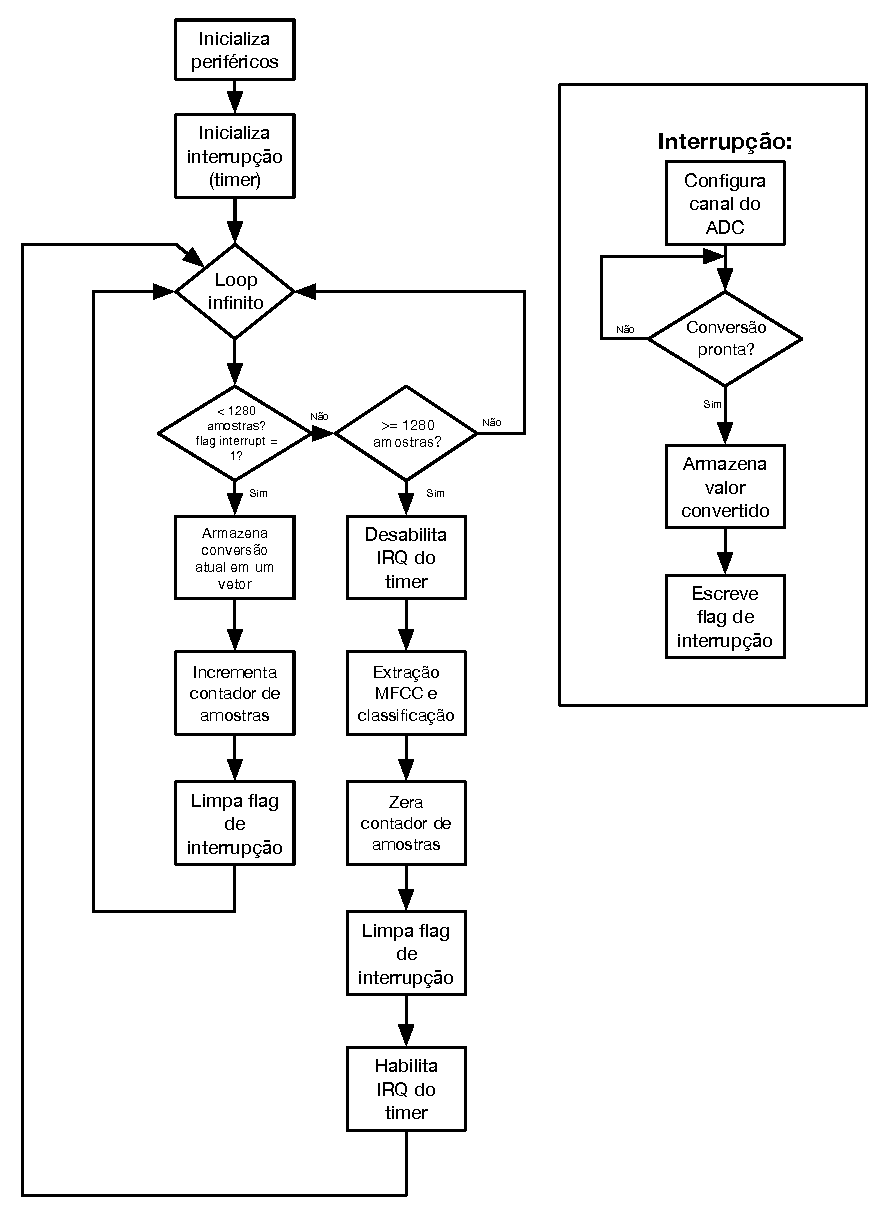
\includegraphics[width=0.5\textwidth]{../Diagramas/FluxoAplicacao}
	\caption{Fluxo da aplicação implementada}
	\label{fig:fluxoaplicacao}
\end{figure}

\section{Resultados}

\subsection{Testes de captura e processamento}

O sistema foi programado com a aplicação apresentada na figura \ref{fig:fluxoaplicacao}.

Executaram-se testes onde, exposto a uma fonte sonora que reproduzia amostras de choro, o protótipo enviava ao computador, via conversor serial-USB externo, os coeficientes calculados.

Para verificar a integridade da captura das amostras, também foram executados testes onde enviava-se, via serial, o vetor com os valores capturados diretamente pelo conversor analógico-digital, dados que permitiram a visualização do sinal capturado no domínio do tempo.

Nestes testes, utilizou-se o chaveamento de um LED para, com o auxílio de um osciloscópio digital, determinar o tempo de duração de cada parte do programa.

A rotina que captura as 1280 amostras e as armazena em um vetor durou 80ms, enquanto o processamento para extração das características levou 15ms.


\subsection{Reconhecimento de choro}

O treinamento da rede neural utilizando os coeficientes obtidos utilizou 45580 \textit{frames} de choro infantil para entrada (amostras positivas, às quais foi atribuída a classe 1), e 201019 \textit{frames} contendo ruídos diversos, como ruídos de construção civil, movimento de automóveis, sirenes e vozes humanas sobrepostas (amostras negativas, às quais atribuiu-se a classe 0).

Para determinar o número de neurônios ocultos, repetiu-se o treinamento em várias iterações, variando de 2 a 20 neurônios.

\subsection{Discussão dos resultados}

Como medida de desempenho do sistema, utilizou-se a interpretação de uma matriz de confusão.

Uma matriz de confusão  apresenta o desempenho de um classificador em uma tabela simples:

\begin{table}[H]
\centering
\begin{tabular}{ccc|l}
\cline{2-3}
\multicolumn{1}{c|}{n = 190}       & \multicolumn{1}{c|}{Previsto 0}                 & Previsto 1                 &                                                  \\ \cline{1-3}
\multicolumn{1}{|c|}{Verdadeiro 0} & \multicolumn{1}{c|}{\cellcolor[HTML]{9AFF99}60} & \cellcolor[HTML]{FFCCC9}25 &                                                  \\ \cline{1-3}
\multicolumn{1}{|c|}{Verdadeiro 1} & \multicolumn{1}{c|}{\cellcolor[HTML]{FFCCC9}15} & \cellcolor[HTML]{9AFF99}90 &                                                  \\ \hline
\multicolumn{1}{l}{}               & \multicolumn{1}{l}{}                            & \multicolumn{1}{l|}{}      & \multicolumn{1}{l|}{\cellcolor[HTML]{CBCEFB}150} \\ \cline{4-4} 
\end{tabular}
\caption{Exemplo de matriz de confusão}
\label{tab:confusao_exemplo}
\end{table}

A tabela \ref{tab:confusao_exemplo} mostra um exemplo de matriz de confusão para uma classificação binária de 190 entradas. Destas, 60 entradas que pertenciam à classe 0 foram corretamente classificadas e 25 entradas que pertenciam à classe 0 foram incorretamente classificadas como sendo da classe 1, 15 entradas da classe 1 foram incorretamente classificadas como sendo da classe 0 e 90 entradas da classe 1 foram corretamente classificadas. A última célula mostra o valor total de acertos.

Após o treinamento realizado com diferentes números de neurônios, as matrizes de confusão dos melhores resultados obtidos são apresentados nas figuras \ref{fig:confusao1}, \ref{fig:confusao2} e \ref{fig:confusao3}.
\begin{figure}[H]
	\centering
	\includegraphics[scale=0.43]{img/confusao_8neuron}
	\caption{Matriz de confusão para 8 neurônios ocultos}
	\label{fig:confusao1}
\end{figure}

\begin{figure}[H]
	\centering
	\includegraphics[scale=0.43]{img/confusao_10neuron}
	\caption{Matriz de confusão para 10 neurônios ocultos}
	\label{fig:confusao2}
\end{figure}

\begin{figure}[H]
	\centering
	\includegraphics[scale=0.43]{img/confusao_16neuron}
	\caption{Matriz de confusão para 16 neurônios ocultos}
	\label{fig:confusao3}
\end{figure}

Como a implementação do classificador é feita num sistema com memória limitada, é coerente escolher o melhor resultado com menor número de neurônios.

Na figura \ref{fig:confusao1}, as primeiras duas células diagonais da matriz de confusão indicam que 198920 amostras, correspondentes a 80,7\% do total, foram classificadas corretamente como 0 (não houve choro) e 41033 amostras, 16,6\% do total, foram classificadas corretamente como 1 (houve choro). Ainda, indica-se que 4547 amostras (1,8\% do total) foram incorretamente classificadas como 0 (\textit{não houve choro}) e 2099 (0,9\% do total) foram classificadas incorretamente como 1 (\textit{houve choro}).

A figura \ref{fig:confusao1} ainda indica que, de 203467 predições 0 (soma das duas primeiras células, $ 198920 + 4547 $), 97,8\% foram classificadas corretamente. Na linha abaixo, indica-se que, de 43132 predições 1 ($ 2099 + 41033 $), 95,1\% foram corretamente classificadas. A última célula da primeira coluna indica que 99\% de 201019 (soma das duas células acima) casos 0 foram corretamente classificados. A última célula da segunda coluna indica que, de 45580 casos 1, 90\% foram classificados corretamente.

Finalmente, a última célula da matriz da figura \ref{fig:confusao1} mostra que, no geral, 97,3\% das previsões foram corretas.

\section{Conclusão e trabalhos futuros}

Este trabalho apresentou a possibilidade de implementação de um sistema de reconhecimento de choro infantil em um microcontrolador de baixo custo e potência.

A utilização de redes neurais para classificação permitiu que a detecção funcionasse mesmo em casos onde algum fator variava, como a distância entre a criança e o microfone.

Ainda, a extração dos coeficientes cepstrais na frequência mel permitiu melhor caracterização das vocalizações produzidas durante o choro. Este método pode ser estendido para detectar além da ocorrência do choro, a sua motivação. Se forem obtidas amostras ligadas a reações da criança, como fome, dor ou desconforto, pode-se treinar a rede neural para identificar diferenças entre os choros que expressam cada sensação, o que pode ser útil no tratamento com a criança.

Ademais, o funcionamento do receptor pode ser estendido para receber sinais de outros dispositivos, que podem ser integrados em uma rede local utilizando protocolos de rede para aplicações residenciais.

\section*{Agradecimentos}
O autor agradece à empresa Incluir Tecnologia pela permissão de realizar e abordar o desenvolvimento do projeto.

\printbibliography

\end{multicols*}
\end{document}
